% **********************************************************************
% Copyright 2020 Aleksander GRM

% Author: Aleksander GRM @fpp.uni-lj.si
% Description: This is an unofficial book tmplate I made from scratch. 
%              Feel free to use it, modify it, share it.
% Version: 1.0
% Date: 02/12/2020
% **********************************************************************


% ******************
% *** page style ***
%
\documentclass[10pt,twosided]{book}
%
% ******************


% ******************************************
% *** hyper references must be set first ***
% ******************************************
%
% *** choose a correct version with used compiler ***
%
%\usepackage[dvips]{hyperref}  % latex + dvips + ps2pdf
%\usepackage[pdftex]{hyperref} % pdflatex
\usepackage[xetex]{hyperref}   % xelatex (default)
\hypersetup{
	colorlinks = true,
	linkcolor = {red!50!black},
	citecolor = {blue!50!black},
	urlcolor = {blue!80!black}
}


% ********************************************************
% *** Compile with xelatex requires UTF-8 file format! ***
% ********************************************************
% 
% *** UTF-8 coding
% 
% Comment if copiled with xelatex, unless uncomment for pdflatex!
%
%\usepackage[utf8x]{inputenc} % needed for pdflatex


% ************************
% *** Language support ***
% ************************
%
\usepackage[slovene]{babel}
%\usepackage[english]{babel}
% ************************


% *** show labels ***
% \usepackage{showlabels}

% *********************
% *** Paper margins ***
% *********************
%
\usepackage{geometry}
\geometry{
	paperwidth=160mm,
	paperheight=225mm,
	left=25mm,
	width=115mm,
	top=25mm,
	height=180mm
}
%
% *** Crop marks ***
%
%\usepackage[a4,frame,center]{crop}
\usepackage[a4,cam,center]{crop}

%
% *** Fancy chapter/section look ***
%
%Options: Sonny, Lenny, Glenn, Conny, Rejne, Bjarne, Bjornstrup
\usepackage[Bjornstrup]{fncychap}
%
\usepackage{titlesec}
\titleformat{\section}
{\normalfont\sffamily\Large\bfseries}
{\thesection}{1em}{}
\titleformat{\subsection}
{\normalfont\sffamily\large\bfseries}
{\thesubsection}{1em}{}


%
% *** include packages ***
%
\usepackage[numbers]{natbib}
\usepackage{parskip}
\usepackage{graphicx}
\usepackage{xcolor}
\usepackage{subfigure}
\usepackage{multicol}
\usepackage{mathtools}
\usepackage{amsmath,amsthm,amssymb,latexsym}
\usepackage{empheq, nccmath}
\usepackage[many]{tcolorbox}
\usepackage{siunitx}
\usepackage{datetime}
\usepackage{fancyhdr}
\usepackage{emptypage}
%
% registered - \textregistered
% copyright  - \textcopyright
\usepackage{textcomp}

%
\usepackage[all,knot]{xy}
\xyoption{arc}
\usepackage{multimedia}
\usepackage{setspace}
\usepackage{listings}
\usepackage{textcomp}
\usepackage{bm}
\usepackage{xfrac}
\usepackage{cancel}

%
% *** Drawing tools ***
%
\usepackage{tikz}
\usetikzlibrary{shadings}
\usetikzlibrary{calc} 

%
% *** Matlab
\usepackage[framed,numbered]{matlab-prettifier}

%
% *** Caption to be bold face ***
%
\usepackage{caption}
\captionsetup[figure]{labelfont=bf}


%
% *** Numbered environment ***
%
%\newenvironment{naloga}[1][]{\noindent \textbf{Naloga} }{\medskip}
\newenvironment{primer}[1][]{\noindent \textbf{Primer.}  }{\medskip}
\newenvironment{resitev}[1][]{\noindent \textbf{Rešitev.}  }{\medskip}

%
% *** Examples ***
%
\theoremstyle{definition}
\newtheorem{exmp}{}[section]
\newtheorem{naloga}{Naloga}[section]


%
% *** Fancy header ***
%
\renewcommand{\chaptermark}[1]{\markboth{\chaptername\ \thechapter.\ #1}{}}
\renewcommand{\sectionmark}[1]{\markright{\thesection.\ #1}}  
%
\pagestyle{fancy}
\fancyhf{}
\fancyhead[LE]{\itshape\nouppercase\leftmark}
\fancyhead[RE]{\textsc{A.Grm}\copyright2022}
\fancyhead[RO]{\itshape\nouppercase\rightmark}
\fancyhead[LO]{\textsc{A.Grm}\copyright2022}
\chead{}
\cfoot{\thepage}

% ********************************
% *** Additional notations.tex ***
% ********************************
%
% 
%       *** Latex additions ***
% 
% - Author: aleksander.grm@fpp.uni-lj.si 
% - Date: 04/12/2023 (last modified)

%
% *** Needed packages ***
%
\usepackage{dsfont}

%
% *** New Commands ***
%
%\newcommand*{\point}[1]{\vec{\mkern0mu#1}}
\newcommand{\ci}[0]{\perp\!\!\!\!\!\perp} % conditional independence
\newcommand{\point}[1]{{#1}} % points 
\renewcommand{\vec}[1]{\boldsymbol{#1}}  % math vector
\newcommand{\uvec}[1]{\mathbf{\hat{#1}}} % unit vector
%\newcommand{\mat}[1]{\boldsymbol{#1}}    % matrix
\newcommand{\mat}[1]{\boldsymbol{\mathsf{#1}}}    % matrix
\newcommand{\RR}[0]{\mathbb{R}} % real numbers
\newcommand{\ZZ}[0]{\mathbb{Z}} % integers
\newcommand{\NN}[0]{\mathbb{N}} % natural numbers
\newcommand{\QQ}[0]{\mathbb{Q}} % rational numbers
\newcommand{\CC}[0]{\mathbb{C}} % complex numbers
\newcommand{\tr}[0]{\text{tr}} % trace
\renewcommand{\d}[0]{\mathrm{d}} % total derivative
\newcommand{\prt}[0]{\partial}
\newcommand{\inv}{^{-1}} % inverse
\newcommand{\id}{\mathrm{id}} % identity mapping
\renewcommand{\dim}{\mathrm{dim}} % dimension
%\newcommand{\dim}[1]{\text{\textsc{dim}}\left(#1\right)} 
\newcommand{\adj}[1]{\mathrm{adj}(#1)} % adjoint or adjugate matrix
\newcommand{\rank}[1]{\mathrm{rk}(#1)} % rank
\newcommand{\determ}[1]{\mathrm{det}(#1)} % determinant
%\renewcommand{\det}[1]{\mathrm{det}(#1)} % determinant
\newcommand{\scp}[2]{\langle #1 , #2 \rangle}
\newcommand{\kernel}[1]{\mathrm{ker}({#1})} % kernel/nullspace
\newcommand{\img}[0]{\mathrm{Im}} % image
\newcommand{\idx}[1]{{(#1)}} % index
\newcommand{\diag}[1]{{\mathrm{diag}(#1)}} % diagonal operator
\newcommand{\cov}[1]{{\mathrm{cov}(#1)}} % covariance (matrix) 
\newcommand{\mean}{\mathds{E}} % expectation
\newcommand{\var}{\mathds{V}} % variance
\newcommand{\gauss}[2]{\mathcal{N}\big(#1,\,#2\big)} % gaussian distribution N(.,.)
\newcommand{\gaussx}[3]{\mathcal{N}\big(#1\,|\,#2,\,#3\big)} % gaussian distribution N(.|.,.)
\newcommand{\gaussBig}[2]{\mathcal{N}\left(#1,\,#2\right)} % see above, but with brackets that adjust to the height of the arguments
\newcommand{\gaussxBig}[3]{\mathcal{N}\left(#1\,|\,#2,\,#3\right)} % see above, but with brackets that adjust to the height of the arguments

\newcommand{\T}[0]{^\top} % transpose
\newcommand{\imu}[0]{\mathrm{i}} % complex unit i
\newcommand{\matdet}[1]{\left|\begin{matrix}#1\end{matrix}\right|} % determinant of a matrix
\newcommand{\vecnorm}[1]{\lVert#1\rVert}
\newcommand{\absval}[1]{\lvert#1\rvert}
\newcommand{\scaprod}[2]{\langle #1, #2 \rangle_0}
\newcommand{\operator}[2]{\operatorname{#1}\left[#2\right]}
\newcommand{\order}[2]{\mathcal{O}({#1}^{#2})}

%
% *** Arc notations ***
%
\newcommand{\txtdeg}{\si{\degree}}
\newcommand{\txtmin}{\si{\arcmiute}}
\newcommand{\txtsec}{\si{\arcsecond}}
\newcommand{\arcdeg}[1]{\si{\ang{#1;;}}}
\newcommand{\arcmin}[1]{\si{\ang{;#1;}}}
\newcommand{\arcsec}[1]{\si{\ang{;;#1}}}
\newcommand{\posdm}[2]{\si{\ang{#1;#2;}}}
\newcommand{\posdms}[3]{\si{\ang{#1;#2;#3}}}

%
% *** some shotcuts, bolded symbols, fnacy style, ... ***
%
\newcommand{\mc}{\mathcal}
\newcommand{\mb}{\mathbb}
\newcommand{\ul}{\underline}
\newcommand{\tb}{\textbf}
\newcommand{\bk}{\boldkey}
\newcommand{\bs}{\boldsymbol}
\newcommand{\circled}[1]{\tikz[baseline=(char.base)]{\node[shape=circle,draw,inner sep=1pt] (char) {#1};}}

%
% *** Special keywords
%
\newcommand{\cpp}{\textbf{\texttt{c++}}}
\newcommand{\python}{\textbf{\texttt{python}}}

%
% *** dimension less numbers, and other numbers ***
%
\newcommand{\RE}{\text{\textsl{Re}}}
\newcommand{\MA}{\text{\textsl{Ma}}}
\newcommand{\KN}{\text{\textsl{Kn}}}
%\newcommand{\half}{\sfrac{1}{2}}
\newcommand{\half}{1/2}
\newcommand{\emphc}[1]{\textcolor{deepcarminepink}{\textbf{#1}}}

%
% *** tabular ***
%
\newcommand{\centercell}[1]{\multicolumn{1}{c}{#1}}
\newcommand{\head}[1]{\centercell{\bfseries#1}}

%
% *** various color definitions ***
%
\definecolor{darkgreen}{rgb}{0,0.6,0}
%
\newcommand{\blue}[1]{{\color{blue}#1}}
\newcommand{\red}[1]{{\color{red}#1}}
\newcommand{\green}[1]{{\color{darkgreen}#1}}
\newcommand{\orange}[1]{{\color{orange}#1}}
\newcommand{\magenta}[1]{{\color{magenta}#1}}
\newcommand{\cyan}[1]{{\color{cyan}#1}}
%
\definecolor{royalblue1}{RGB}{72,118,255}
\definecolor{shadowbg}{RGB}{51,51,51}
\definecolor{titlebg}{RGB}{51,51,51}
\definecolor{royalblue4}{RGB}{39,64,139}
\definecolor{navyblue}{RGB}{0, 0, 127}
\definecolor{deepcarminepink}{rgb}{0.94, 0.19, 0.22}

%
% *** redefine EMPH types ***
%
\renewcommand{\emph}[1]{\blue{\bf{#1}}}
\newcommand{\myfig}[1]{\iflanguage{english}{\textbf{Figure}}{\textbf{Slika}} #1}
\newcommand{\myeq}[1]{\iflanguage{english}{\textbf{Eq.}}{\textbf{En.}} (#1)}

%
% *** place a colored box around a character ***
%
\gdef\colchar#1#2{%
	\tikz[baseline]{%
		\node[anchor=base,inner sep=2pt,outer sep=0pt,fill = #2!20] {#1};
	}%
}%

%
% *** Trade names, Copy right... ***
%
% \textsuperscript \textsubscript
\newcommand{\matlab}{\textit{\texttt{MatLab}}\textsuperscript{\textregistered} }
\renewcommand{\python}{\textit{\texttt{Python}}\textsuperscript{\textregistered} }
\newcommand{\numpy}{\textit{\texttt{NumPy}}\textsuperscript{\textregistered} }
\newcommand{\scipy}{\textit{\texttt{SciPy}}\textsuperscript{\textregistered} }
\newcommand{\mplpy}{\textit{\texttt{MatPlotLib}}\textsuperscript{\textregistered} }
\newcommand{\sage}{\textit{\texttt{SageMath}}\textsuperscript{\textregistered} }


% ***********************************************
% *** Blocks: block, exampleblock, alertblock ***
% ***********************************************

%
% *** Blocks: block, exampleblock, alertblock ***
%
%\definecolor{shadowbga}{RGB}{51,51,51}
\definecolor{myblue}{rgb}{.9, .9, 1}
\definecolor{lightblue}{rgb}{.9, .9, .5}
%\newcommand*\mybluebox[1]{%
	%	\colorbox{myblue}{\hspace{1em}#1\hspace{1em}}}

\newlength\mytemplen
\newsavebox\mytempbox

\makeatletter
\newcommand\mybluebox{%
	\@ifnextchar[%]
	{\@mybluebox}%
	{\@mybluebox[0pt]}}

\def\@mybluebox[#1]{%
	\@ifnextchar[%]
	{\@@mybluebox[#1]}%
	{\@@mybluebox[#1][0pt]}}

\def\@@mybluebox[#1][#2]#3{
	\sbox\mytempbox{#3}%
	\mytemplen\ht\mytempbox
	\advance\mytemplen #1\relax
	\ht\mytempbox\mytemplen
	\mytemplen\dp\mytempbox
	\advance\mytemplen #2\relax
	\dp\mytempbox\mytemplen
	\colorbox{myblue}{\hspace{1em}\usebox{\mytempbox}\hspace{1em}}}
\makeatother


% *** Example Boxed Equation ***
%

% For a single line equation use: box={\mybluebox[5pt][-2pt]}

% \begin{empheq}[box=\mybluebox]{equation*}
	%   c(t) = c_{in}\left[ 1 - \left(1+ \frac{\Delta \phi}{V_0} \: t
	%   \right)^{-\frac{\phi_{in}}{\Delta \phi}} \right]
	% \end{empheq}
%
% \begin{empheq}[box={\mybluebox[5pt]}]{equation*}
	% 	c_i = \sum_j A_{ij}
	% \end{empheq}
%
% \begin{empheq}[box={\mybluebox[5pt][-2pt]}]{equation*}
	%	c_i = \langle\psi|\phi\rangle
	% \end{empheq}


% *********************************************************
% *** Inline code listings: Matlab, Python pretty print ***
% *********************************************************

\usepackage{listings}
\usepackage{xcolor}

\definecolor{codegreen}{rgb}{0,0.6,0}
\definecolor{codegray}{rgb}{0.5,0.5,0.5}
\definecolor{codepurple}{rgb}{0.58,0,0.82}
\definecolor{backcolour}{rgb}{0.95,0.95,0.92}

\lstdefinestyle{mystyle}{
	backgroundcolor=\color{backcolour},   
	commentstyle=\color{codegreen},
	keywordstyle=\color{magenta},
	numberstyle=\tiny\color{codegray},
	stringstyle=\color{codepurple},
	basicstyle=\ttfamily\footnotesize,
	breakatwhitespace=false,         
	breaklines=true,                 
	captionpos=b,                    
	keepspaces=true,                 
	numbers=left,                    
	numbersep=5pt,                  
	showspaces=false,                
	showstringspaces=false,
	showtabs=false,                  
	tabsize=2
}


% *** Example ***
 
% language: Matlab-editor, Matlab-Pyglike, Python, Octave, C, C++,
% look in help doc for additional languages  

%\begin{frame}[fragile]{Title}
%
%  \lstinputlisting[language=Octave,style=mystyle]{BitXorMatrix.m}
%
%\end{frame}


% ******************************
% *** Definicija slo za math ***
% ******************************
\newtheorem{izrek}{Izrek}
\newtheorem{lema}[izrek]{Lema}
\newtheorem{trditev}[izrek]{Trditev}
\newtheorem{posledica}[izrek]{Posledica}
\newtheorem{definicija}[izrek]{Definicija}
\newtheorem{vaja}[izrek]{Vaja}




%
% *********************

%\AtBeginShipout
%{
%	\begin{tikzpicture}[remember picture,overlay]
%		\node [rectangle, anchor=north, minimum width=9cm, minimum height=\paperheight+1cm] (box) at (-5cm,0.5cm){};
%	\end{tikzpicture}
%}

\begin{document}
%%%%%%%%%%%%%%%%%%%%%%%%%%%%%%%%%%%%%%%%%%%%%%%%%%%%%%%%%%%%%%%%%%%%%%%%%%%%%%%%%%%%%%%%%
\pagenumbering{roman}
\pagestyle{empty}

    \begin{center}
	    
\includegraphics[height=5cm]{fpp_logo_vertical_slo_red.pdf}\\[3cm]
	    
		\rule{\linewidth}{1 mm} \\[7mm]
		{ \huge \bfseries Oceanska navigacija}\\[4mm]
		\rule{\linewidth}{1 mm} \\[3cm]
		
		{\large \textsc{Aleksander Sandro GRM} }\\[2mm]
		{\large \textsc{Tanja BRCKO SATLER} }
		
		\vspace{3cm}
		2022, 1. izdaja
		
	\end{center}

\clearpage
~
%%%%%%%%%%%%%%%%%%%%%%%%%%%%%%%%%%%%%
\newpage
\pagestyle{plain}
\setcounter{page}{1}

\tableofcontents

% ***********************************
\newpage
\chapter*{Povzetek}

Pričujoča knjiga je namenjena predvsem študentom pomorske smeri na Fakulteti za pomorstvo in promet, Univerze v Ljubljani. Hkrati pa vabi vse zanesenjake, ki jih zanima klasičen način določanja položaja na odprtem morju. Knjiga je vsebinsko podana na način, da se lahko vsakdo, ki ima nekaj predznanja matematike, fizike in astronomije, sam priuči opisanih metod določevanja položaja. Kar potrebuje, je le sekstant, podatke o nebesnih telesih, žepni računalnik, pričujočo knjigo in dobro voljo.

Mogoče bi še kdo ob teh besedah pripomnil, da je danes v uporabi satelitska navigacija in se metode klasične Oceanske navigacije na ladjah trgovske mornarice ne uporabljajo več. Tudi to bo držalo, vendar ne v celoti. Bistvo STCW usposabljanja \cite{cfd_ferziger_peric} temelji tudi na avtonomnosti navigacijskih načel in principov, kjer je poglavje oceanske navigacije pomemben del STCW vsebin. Tako morajo vsi pomorščaki še vedno znati določiti položaj na odprtem morju z uporabo klasičnih metod, kot so avtonomni sistemi navigacije brez napajanja. Popolnoma jasno je tudi zakaj mora biti tako. V današnjem času se vse bolj dogaja, da se položaj določen s pomočjo satelitov moti in je kot takšen nezanesljiv, vendar izjemno natančen. Kombinacija obeh sistemov prinaša zanesljivost in hkrati natančnost, ter tako izpolnjuje osnovna načela SOLAS konvencije.

Vsebina knjige se podaja po poti praktične navigacije, kakor jo je zasnoval kapitan \textit{Nathaniel
Bowditch} v svoji knjigi \textit{American Practical Navigator} \cite{cfd_ferziger_peric}. Načelo kapitana Bowditch je: \textit{"Vsak pomorščak se lahko nauči in priuči osnovnih principov navigacije."} Za izpolnitev take ideje, potrebujejo pomorščaki kvalitetno literaturo. Osnovna literatura mora vsebovati teoretično podlago, kjer lahko bralec sledi poti razvoja od osnovnih principov do uporabne forme, ki je nato podlaga praktičnega pomorskega usposabljanja.

\vspace{2mm}
\begin{flushright}
	-- Aleksander Sandro GRM --\\[2mm]
	-- Tanja BRCKO SATLER --\\[2mm]
	-- September, 2023 --
\end{flushright}  
\clearpage
~
%%%%%%%%%%%%%%%%%%%%%%%%%%%%%%%%%%%%%%
\newpage
\pagestyle{fancy}
\pagenumbering{arabic}
\setcounter{page}{1}

\chapter{Uvod}

Začetki sodobne oceanske navigacije segajo v obdobje petnajstega stoletja, ko je odprava Ferdinanda Magelana prvič obplula svet. Na tem potovanju je žal kapitan Magelan tragično izgubil življenje na Filipinih v boju za Mactan (1521). Ladja Victorija se tako vrne brez vodje odprave in prvič v evropski sodobni zgodovini obpluje svet.

To obdobje je obdobje junakov in pionirjev, ki so prvi odkrivali svet s plovbo po širnih oceanih. Pri navigaciji so si pomagali s primitivnimi navigacijskimi pripomočki, kakor so tedaj vedeli in znali. Velikokrat se je zgodilo, da niso vedeli kje so, oziroma se jim je le dozdevalo kje so. To so bili časi navigacije, ko je bilo še veliko v rokah vsemogočnega Pozejdona ali Neptuna in pomočnika za veter Aeolusa. 

Velik napredek v oceanski navigaciji pride s kasnejšimi odpravami Vasco de Gama, Francis Drage in James Cook. Prav izum kronometra, bolj natančno ladijskega kronometra z oznako H-4, ki ga je izumil John Harrison, sekstanta, kot ga danes poznamo, ki ga je izdelal John Hadley in navtičnega almanaha, se je pričelo moderno obdobje oceanske oziroma astronomske navigacije.

Principi sodobne oceanske navigacije temeljijo na sferni trigonometriji. Da bi lahko določili naš položaj na oceanu, ali s pomočjo meritve časa in hitrosti ali s pomočjo meritve višine nebesnih teles, vseskozi potrebuje način preračun s katerim določimo položaj opazovalca. Velik del potrebnih enačb so prav enačbe sferne trigonometrije, ki jih potrebujemo za določitev položaja opazovalca s pomočjo podatkov meritev. Prvo poglavje knjige je zato namenjeno predstavitvi sferne trigonometrije. Prikaže se postopek izpeljave osnovnih izrekov sferne trigonometrije iz osnovnih matematičnih principov. Čeprav v določenih primerih, opis problema s pomočjo sfere ni najbolj natančen, je pa še vedno zelo natančen za uporabo v pomorstvu. S to natančnostjo bomo v večino primerih tudi zadovoljni.

Naslednja poglavja razpredajo o osnovah plovbe po Zemlji kot sferi, kjer poteka razlaga pojmov \emph{loksodromske} in \emph{ortodromske} plovbe. V začetku si pogledamo osnove cilindrične in Merkatorjeve projekcije zemeljske oble na ravnino, ki jo imenujemo pomorska karta. Vsak pomorščak mora znati izdelati tako imenovano \emph{belo karto}, to je Merkatorjevo karto za določeno geografsko področje. Tako sledi opis postopka izdelave Merkatorjeve karte. Poglavje se zaključi z izdelavo plana potovanja. 

V naslednjem poglavju so razložene osnove astronomske navigacije, z opisom vseh klasičnih metod določanja parametrov položaja opazovalca. Najbolj poznana med njimi je \emph{višinska metoda} ali metoda \emph{Marcq de Saint-Hilaire}, imenovana po njenem izumitelju, admiralu  \emph{Marcq de Blond de Saint-Hilaire} \cite{duval1966admiral}. V začetku pričnemo z obravnavo koordinatnih sistemov, ki so temelj izdelave astronomskega navtičnega trikotnika. Nato se posvetimo obravnavi časa in časovnih kotov, ki so posledica gibanja Zemlje. Pri določevanju položaja opazovalca merimo višino nebesnega teles, ki jo je potrebno popraviti zaradi različnih napak. Opišejo se napake in postopki korekcije. Vsi astronomski podatki o nebesnih telesih so združeni v \emph{Efemeridah}, ki so del \emph{Navtičnega almanaha}. Efemeride so lahko v papirnati ali digitalni obliki. Oboji vsebujejo specifične podatke, ki jih navigator potrebuje za določitev astronomskega položaja. Sledijo opisi in prikazi uporabe različnih metod določanja položaja. Poglavje zaključimo z obravnavo vzhoda in zahoda nebesnih teles, ter praktično uporabo pri določanju napake kompasa.

V zadnjem poglavju je opisan pregled uporabe računalnikov, tablic in telefona za uporabo v Oceanski navigaciji. Danes, je večino računskih postopkov digitaliziranih in posplošenih z uporabo naprednih algoritmov za določanje položaja opazovalca. Prikazali bomo uporabo določenih sistemov in razložili ozadje delovanja. Kot podpora k poglavju sodi tudi dopolnilno poglavje, ki vsebuje opis specifičnih komponent računalniških programov. Programi so delo avtorja ali pa pridobljeni iz spleta.  


\newpage
\chapter{Sferna trigonometrija}

Oceanska navigacija, je navigacija, ki poteka na odprtem morju in na \emph{velikih razdaljah}. Recimo tipičen primer je tako plovba med Ameriko in Azijo, kot je prikazana na sliki \ref{fig:02-01-ortodorma_loksodroma}. Na slik \ref{fig:02-01-ortodorma_loksodroma}a se takoj opazi, da je najkrajša pot tista \textit{čudna} pot, ki je na Merkatorjevi navigacijski karti (slika \ref{fig:02-01-ortodorma_loksodroma}b) prikazana kot ukrivljena pot, ki jo imenujemo \emph{Ortodroma}. 

	\begin{figure}[!htpbp]
		\begin{minipage}[t]{55mm}
			(a)
			\vspace{2mm}
			\begin{center}
				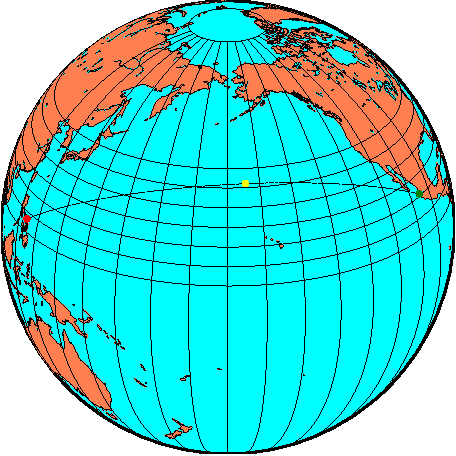
\includegraphics[width=55mm]{02_st/figs/fig_02_01-gc_path.pdf}
			\end{center}
		\end{minipage}
		\hfill
		\begin{minipage}[t]{55mm}
			(b)
			\vspace{2mm}
			\begin{center}
				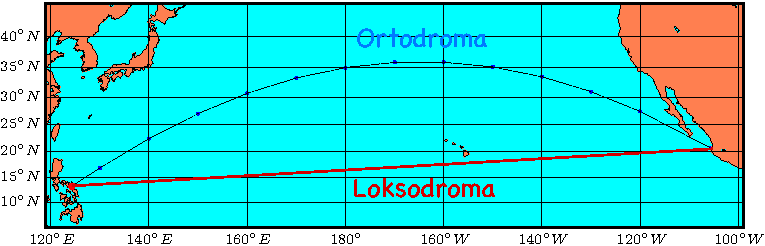
\includegraphics[width=55mm]{02_st/figs/fig_02_02-gc_RL-path.pdf}
			\end{center}
		\end{minipage}
		\caption{Prikaz razlike med potjo po krožnici--\textit{Ortodroma} in potjo po liniji--\textit{Loksodromi}, ki seka meridiane vedno pod istim kotom.}
		\label{fig:02-01-ortodorma_loksodroma}
	\end{figure}

Lepa pot med točko odhoda in točko prihoda, ki je prikazana na sliki \ref{fig:02-01-ortodorma_loksodroma}b kot ravna je ravna črta, je pot, ki ji pravimo \emph{Loksodroma}. Primera pokažeta, da je obvladovanje in razumevanje krivulj, ki potekajo po sferi, zelo pomembna vsebina na področju oceanske navigacije. 

Motivacija razlage in uporabe sferne trigonometrije je povezana predvsem z kombinacijo različnih lokov, ki potekajo po sferi. V večno primerih so loki, ki so deli \emph{velike krožnice}. Pomen le teh, bo razložen kasneje. 


\section{Kratka zgodovina razvoja}

Začetki sferne trigonometrije segajo že daleč v preteklost. Zgodovinarji pravijo, da so probleme sferne trigonometrije obravnavali že stari Indijci in Kitajci. Nam bližje je delo starih Grkov, \textit{Menelausa iz Aleksandrije}, ki v svojem delu \textit{Sphaerica} obravnava sferno trigonometrijo in prikaže razpravo o geodetkah, kjer se ukvarja z izračunom dolžine lokov, ki potekajo po sferi. Tudi zelo znan grški matematik \textit{Evklid} se je ukvarjal s problemi sferne trigonometrije. V svojih razpravah je tako pričel z osnovami razvoja kosinusnega izreka v sferni trigonometriji.

Različne razprave o sferni trigonometriji, so kasneje prispevali arabski matematiki. Recimo \textit{Abu Nasri Mansur ibn Ali ibn Iraq}, ki je bil študent zanega arabskega matematika \textit{Abū al-Wafā Būzhjānī}, je izpeljav sinusni izrek za sferni trikotnik. Kasneje so sledila še druga odkritja različnih zakonov in identitet sferne trigonometrije. Motivacija je bila določitev smeri, iz kraja opazovalca do stavbe \textit{Kabba}, ki je center muslimanske vere. To je tako imenovani problem \textit{qibla}. V tem problemu je Abu Nasri obravnaval izračun smeri, ki jo določa velika krožnica, ki povezuje kraj opazovalca in pa položaj Kabbe.

Kasneje se v obdobju razsvetljenstva v celoti postavijo aksiomatični temelji sferne trigonometrije, kakor jih poznamo danes. \emph{John Napier} je bil izjemen škotski matematik, ki je tako v 17. stoletju postavil temelje sferne trigonometrije, kot jo poznamo danes. John Napier ni znan samo po sferni trigonometriji, ampak še po obravnavi logaritmov, decimalnem zapisu števil in podobnem.

Kot vidimo skozi kratek zgodovinski opis, se je sferna trigonometrija, kot jo poznamo danes, razvijala kar nekaj časa.



\section{Osnovne definicije}

Sferna trigonometrija je eno od različnih poglavji matematike. Kot taka, mora temeljiti na osnovnih definicijah, da ja kasnejša razprava jasna in enovita. V tem poglavju bomo tako predstavili in opisali osnovne pojme, ki se pojavljajo v sferni trigonometriji.

\subsection{Velika in mala krožnica}

Pričnimo z definicijo majhne in velike krožnice, ki poteka po sferi. Kot je prikazano na sliki \ref{fig:02-02-small_great_circle} je opaziti, da je krožnica na sferi določena kot presečna krivulja med ravnino in sfero. V tem primeru ločimo dva primera:

\begin{itemize}
	\item \emphc{velika krožnica} (great circle): v tem primeru ravnina \emph{poteka skozi center sfere} in je tako presečna krivulja med ravnino in sfero vedno krožnica, ki ima radij \emph{enak} radiju sfere,
	\item \emphc{mala krožnica} (small circle): v tem primeru ravnina \emph{ne poteka skozi center sfere} in je tako presečna krivulja med ravnino in sfero vedno krožnica, ki ima radij \emph{manjši} kakor je radij sfere. 
\end{itemize}

\begin{figure}[!htpbp]
	\begin{center}
		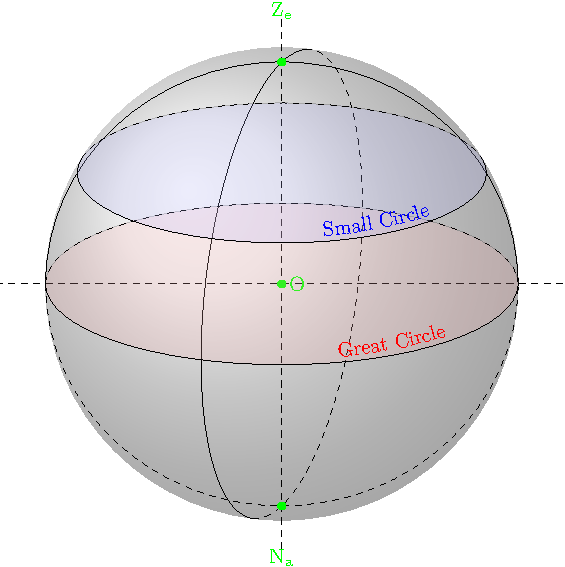
\includegraphics[width=80mm]{02_st/figs/fig_02_03-small_great_circle.pdf}
	\end{center}
	\caption{Prikaz poteka \textit{velike krožnice} (great circle -- GC) in \textit{male krožnice} (small circle -- SC) na sferi.}
	\label{fig:02-02-small_great_circle}
\end{figure}

Kot bomo videli kasneje, bo zelo pomembna definicija velike krožnice, saj je sferni trikotniki vedno sestavljen iz lokov velikih krožnic.

\subsection{Krožni lok}  

\section{Zakoni sferne trigonometrije}

Uvodne besede ...


\section{Primeri}

\newpage
\chapter{Plan potovanja}

\section{Plovba po loksodromi}
Opis sferne trigonometrije ...

\section{Plovba po ortodromi}

\section{Plan potovanja}

\section{Primeri}

\newpage
\chapter{Astronomska navigacija}

Uvodni opis v astronomsko navigacijo ...

\section{Zgodovinski pregled razvoja astronomske navigacije}

\section{Koordinatni sistemi}

\section{Teorija o času}
\subsection{Meritve časa}
\subsection{Časovni koti}


\section{Korekcije višine nebesnih teles}

\section{Opis sekstant, napake in uporaba}

\section{Navtični almanah}

\section{Navtični sferni trikotnik}

\section{Identifikacija zvezd}

\section{Metode določanja položaja}
\subsection{Summner-jeva metoda}
\subsection{Višinska metoda}
\subsection{Prikaz grafičnega določanja položaja -- Uporaba Plot sheet}

\section{Določanje položaja gibajoče ladje}

\section{Direktne metode}

\section{Vzhod -- Zahod nebesnih teles}
\subsection{Čas in azimut nebesnega telesa}
\subsection{Korekcija napake kompasa}

\section{Primeri}

\newpage
\chapter{Uporaba računalnikov}

Uvodni opis v računske metode določanja plana plovbe in astronomskega položaja ...

\section{Plan potovanja -- enostavni ECDIS}

\section{Elektronski navtični almanah}

\section{Metode računskega določevanja položaja}

\section{Primeri}


\newpage
\chapter{Dopolnilo}

\section{Podrobne izpeljave}

\section{PyEcdis}

\section{AstroPy}


% *** References ***
\newpage

% using natbib package: plainnat, unsrtnat, abbrevnat
\bibliographystyle{plainnat}
\bibliography{literature_db}

\end{document}



